\chapter{Ондуляторное излучение}\label{chap:undulatro_radiation}
В этой главе будет дан вывод излучения релятивистского электрона в $r\omega$-пространстве, движущегося в синусоидальном магнитном поле. Вывод замечателен тем, что даёт результаты из первых принципов --- уравнений Максвелла, а все приближения наглядно прослеживаются по ходу изложения. Приведённые выкладки повторяют подход разработанный в серии работ \cite{geloni2005paraxial} -
%, \cite{geloni2007fourier}, \cite{geloni2015brightness },
 \cite{geloni2006fourier}. В заключении главы будет дан обзор на код SRW, \cite{SRW} - \cite{chubar1998proceedings}, а также даны краткие описания других симуляционных кодов, которые активно используются в научном сообществе для расчёта синхротронного излучения. 
\subsection*{Список используемых обозначений}
\begin{equation}
	\begin{array}{lcl}
	\vec{E} \; \textup{--- вектор электрического поля в $rt$-пространстве}\nonumber\\
	\vec{\overline{E}} \; \textup{--- вектор электрического поля в $r\omega$-пространстве}\\
	\vec{\widetilde{E}} \; \textup{--- огибающая волнового пакета электрического поля в $r\omega$-пространстве}\\
	\vec{\widetilde{E}}_{\bot} \; \textup{--- поперечные компонеты ($x,y$) вектора электрического поля}\\
	\textup{в $r\omega$-пространстве}\\ 
	\widetilde{\rho} \;\textup{и} \; \vec{\widetilde{j}} \; \textup{--- плотность заряда и ток в $r\omega$-пространстве}\\
	\vec{r} \; \textup{--- радиус вектор наблюдателя}\\
	\vec{r'} \; \textup{--- радиус вектор частицы}\\
	\vec{r}_{0} \; \textup{--- радиус вектор точки, где наблюдается излучение}\\
	k_w = 2\pi/\lambda_w \textup{, где $\lambda_w$ --- длина периода ондулятора}\\
	\omega_r \; \textup{--- резонансная частота ондулятора}\\
	$e$ \; \textup{--- заряд электрона}\\
	m_e \; \textup{--- масса электрона}\\
	\end{array}
\end{equation}
\section{Излучение релятивистского электрона в синусоидальном магнитном поле}
\subsection{Уравнение движения электрона в ондуляторе}
Вывод спектра излучения ондулятора начнётся с уравнения движения релятивистского электрона в магнитном поле:
\begin{equation}
	\vec{F} = e[\vec{v} \times \vec{B}],
\end{equation} 
где $e$ --- заряд электрона, а $\vec{v}$ и $\vec{B}$ --- скорость частицы и магнитное поле, соответственно. Уравнение можно переписать в виде:

\begin{equation}
	\label{eq:NewTown}
	\cfrac{d\vec{p}}{dt} = \cfrac{e}{\gamma m_e}[\vec{v} \times \vec{B}],
\end{equation}
где $\gamma$ --- Лоренц-фактор, появившийся из релятивистского импульса. Ось $z$ лежит вдоль направления релятивистского движения электрона и считается что, магнитное поле в ондуляторе $B_0\cos(k_w z)$ направлено вдоль оси $y$, где $k_w$ связана с периодом ондулятора следующим образом $k_w = 2\pi/\lambda_w$. После этого, уравнение~\ref{eq:NewTown} можно переписать в виде:

\begin{equation}
	\label{eq:eq_of_motion}
	\begin{cases}
		\cfrac{d^2 x}{dt^2} = - \cfrac{e B_0}{\gamma m_e}\cfrac{dz}{dt} \cos(k_w z)\\
		\cfrac{d^2 z}{dt^2} = \cfrac{e B_0}{\gamma m_e}\cfrac{dx}{dt} \cos(k_w z),
	\end{cases} 
\end{equation}
далее, один раз интегрируя первое уравнение системы с заменой $dz = \beta cdt$, где $\beta = \|\vec{v}\| /c$, можно получить: 

\begin{equation}
 	\label{eq:dx/dt}
	\cfrac{dx}{dt} = - \cfrac{eB_0}{\gamma m_ek_w} \sin(k_w z).
\end{equation}
Введём коэффициент ондуляторности: $K = \cfrac{eB_0 \lambda_u}{2 \pi m_e c}$.
Подставляя получившийся результат~\ref{eq:dx/dt} во второе уравнение системы~\ref{eq:eq_of_motion} и интегрируя с пределами от $0$ до некоторого $z_0$, получим систему:

\begin{equation}
	\begin{cases}
	\label{eq:eq_of_motion_velocity}
		\cfrac{dx}{dt} = - \cfrac{Kc}{\gamma} \sin(k_w z)\\
		\cfrac{dz}{dt} = \beta c - \cfrac{K^2 c}{2 \gamma^2 \beta}\sin^2(k_w z),
	\end{cases} 
\end{equation}
чтобы получить уравнение на траекторию частицы, ещё раз проинтегрируем оба уравнения и, в итоге, получим:

\begin{equation}
	\begin{cases}
	\label{eq:eq_of_motion_trej}
		x = \cfrac{Kc}{\gamma k_w \beta} \cos(k_w\overline{\beta}ct)\\
		z = \overline{\beta}ct + \cfrac{K^2}{8 \beta^2 \gamma^2 k_w}\sin(2k_w\overline{\beta}ct) 
	\end{cases} 
\end{equation}
Здесь введено обозначение $\overline{\beta}$, которое определяется следующим образом $\overline{\beta}c = \beta c\bigg(1 - \cfrac{K^2}{4 \beta^2 \gamma^2}\bigg)$. Полученные решения будут использоваться при интегрировании уравнений Максвелла.
\subsection{Решение уравнений Максвелла в параксиальном приближении}
Вывод спектра излучения будет проводиться в $r\omega$-пространстве. Уравнения Максвелла в вакууме:
\begin{equation}
	\begin{cases}
		\nabla \cdot \vec{E} = 4\pi \rho\\
		\nabla \cdot \vec{B} = 0\\
		[\nabla \times \vec{E}] = -\cfrac{1}{c} \cfrac{\partial\vec{B}}{\partial t}\\
		[\nabla \times \vec{B}] = \cfrac{4\pi}{c} \vec{j} + \cfrac{1}{c} \cfrac{\partial\vec{E}}{\partial t}.
	\end{cases} 
\end{equation}
Из уравнений тривиально можно получить неоднородное волновое уравнение: 
\begin{equation}
	\label{eq:inhomo_wave_eq_xt}
	c^2 \nabla^2 \vec{E} - \pdv[2]{\vec{E}}{t} = 4\pi c^2 \nabla \rho + 4\pi \pdv{\vec{j}}{t}.
\end{equation}
Это же уравнение представимо в $r\omega$-пространстве. Преобразование Фурье определяется следующим образом:
\begin{equation}
	\label{eq:Fourier_wt}
	\begin{array}{lcl}
		{\overline{f}}(r, \omega) = \displaystyle\int\limits_{-\infty}^{\infty} dt {f}(r, t)\exp[i\omega t],\\
		\\
		{f}(r, t) = \cfrac{1}{2\pi}\displaystyle\int\limits_{-\infty}^{\infty} d\omega {\overline{f}}(r, \omega)\exp[-i\omega t].
	\end{array}
\end{equation}
%Уравнение~\ref{eq:inhomo_wave_eq_xt} в $r\omega$-пространстве выглядит следующим образом:
\begin{equation}
	\label{eq:inhomo_wave_eq_xw}
	\omega^2 \vec{\overline{E}} + c^2 \nabla^2 \vec{\overline{E}} = 4\pi c^2 \nabla  \overline{\rho} - 4i\pi\omega\vec{\overline{j}}.
\end{equation}
Это уравнение можно переписать в приближении медленно меняющейся амплитуды, что есть $\vec{\overline{E}} =  \vec{\widetilde{E}}\exp[i\omega z/c]$
%, в приближении $\cfrac{\partial |\vec{E}|}{\partial z} \ll \cfrac{\omega}{c}|\vec{E}|$
Физический смысл состоит в том, что скорость изменения огибающей волнового пакета много меньше чем осцилляции его наполняющей. Исходя из уравнения~\ref{eq:inhomo_wave_eq_xw}, получается:
\begin{equation}
	\label{eq:wave_slow_vary}
	c^2\bigg(\nabla^2 \vec{\widetilde{E}} + \cfrac{2i\omega}{c}\pdv{\vec{\widetilde{E}}}{z}\bigg)\exp[i\omega z/c] = 4\pi c^2 \nabla  \overline{\rho} - 4i\pi\omega\vec{\overline{j}}.
\end{equation}
Для электрона движущегося в вакууме ток и плотность заряда выражаются через дельта-функцию Дирака:
\begin{equation}
	\begin{array}{lcl}
		\rho(r,t) = -e\delta(\vec{r}- \vec{r'}(t)) = -\cfrac{e}{v_z(z)}\delta(\vec{r}_{\bot}- \vec{r'}_{\bot}(z))\delta(\cfrac{s(z)}{v} - t),\\
		\vec{j}(r,t) = \vec{v}\rho(r,t);
	\end{array}
\end{equation} 
в $r\omega$-пространстве: 
\begin{equation}
	\begin{array}{lcl}
		\overline{\rho}(r,\omega) = -\cfrac{e}{v_z(z)}\delta(\vec{r}_{\bot}- \vec{r'}_{\bot}(z))\exp[\cfrac{iws(z)}{v}],\\
		\overline{\vec{j}}(r,\omega) = \vec{v}\overline{\rho}(r,\omega).	
	\end{array}
\end{equation} 
Подставив Фурье-образы плотности тока и заряда в уравнение~\ref{eq:wave_slow_vary}, получается:
\begin{equation}
	\label{eq:wave_eq}
	\begin{array}{lcl}
		\nabla^2 \vec{\widetilde{E}} + \cfrac{2i\omega}{c}\cfrac{\partial\vec{\widetilde{E}}}{\partial z} = 
		\cfrac{4\pi e}{v_z(z)} \exp[iw\bigg(\cfrac{s(z)}{v} - \cfrac{z}{c}\bigg)]
		\bigg(  
			\cfrac{i\omega}{c^2}\vec{v}(z)
			-\nabla\bigg) \delta(\vec{r}_{\bot} - \vec{r'}_{\bot}(z)).
		
	\end{array}
\end{equation} 
Теперь применимо параксиальное приближение. Здесь учитывается приближение медленно меняющейся амплитуды: $\partial_z |\vec{\widetilde{E}}_{x,y}| \ll \omega /c|\vec{\widetilde{E}}_{x,y}|$, что означает, что огибающая волнового пакета слабо меняется на масштабах длины волны излучения, поэтому второй производной по $z$ можно пренебречь, далее будут рассматривать только поперченные компоненты поля:
\begin{equation}
	\label{eq:wave_slow_vary_parax}
	\begin{array}{lcl}
		\nabla_{\bot}^2 \vec{\widetilde{E}}_{\bot} + \cfrac{2i\omega}{c}\cfrac{\partial\vec{\widetilde{E}}_{\bot}}{\partial z} = 
		\cfrac{4\pi e}{v_z(z)} \exp[iw\bigg(\cfrac{s(z)}{v} - \cfrac{z}{c}\bigg)]\bigg(  
			\cfrac{i\omega}{c^2}\vec{v}_{\bot}(z) 
			-\nabla_{\bot}\bigg) \delta(\vec{r}_{\bot} - \vec{r'}_{\bot}(z)).
	\end{array}
\end{equation} 
Это неоднородное дифференциальное уравнение в частных производных, которое будет решено с помощью функции Грина. Для дифференциального оператора $\partial_t - k\nabla_{2D}^2$ функция Грина есть: $\cfrac{1}{4\pi kt}\exp[-\rho^2/4kt]$. В частности для уравнения~\ref{eq:wave_slow_vary_parax}:
\begin{equation}
	\label{eq:Green_func}
	G(z_0 - z'; \vec{r}_{\bot 0} - \vec{r'}_{\bot}) = 
	- \cfrac{1}{4\pi (z_0 - z')}\exp[i\omega \cfrac{|\vec{r}_{\bot 0} - \vec{r'}_{\bot}|^2}{2c(z_0 - z')}].
\end{equation} 
Интегрирование функции Грина с правой частью уравнения~\ref{eq:wave_slow_vary_parax} даёт решение для распределения поля:
\begin{equation}
	\begin{array}{lcl}
		\vec{\widetilde{E}}_{\bot}(z_0,  \vec{r}_{\bot 0}, \omega) = -\cfrac{e}{c}  \displaystyle\int\limits_{-\infty}^{\infty}\int\limits_{-\infty}^{\infty} dz'd\vec{r'}\cfrac{1}{z_0 - z'}
		\bigg(\cfrac{i\omega}{c^2}\vec{v}_{\bot}(z')
		-\nabla'_{\bot}\bigg) \delta(\vec{r}_{\bot} - \vec{r'}_{\bot}(z'))\times\\
		\exp[iw\bigg( \cfrac{|\vec{r}_{\bot 0} - \vec{r'}_{\bot}|^2}{2c(z_0 - z')} +\cfrac{s(z')}{v} - \cfrac{z'}{c} \bigg)].
	\end{array}	
\end{equation}
Проинтегрировав по $d\vec{r'}$, получается общее решение уравнения~\ref{eq:wave_eq} :
\begin{equation}
	\label{eq:field_in_parax_com}
	\begin{array}{lcl}
		\vec{\widetilde{E}}_{\bot}(z_0,  \vec{r}_{\bot 0}, \omega) = -\cfrac{i\omega e}{c^2}  \displaystyle\int\limits_{-\infty}^{\infty} dz'
		\cfrac{1}{z_0 - z'}
		\bigg(\cfrac{\vec{v}_{\bot}(z')}{c}
		- \cfrac{\vec{r}_{\bot 0} - \vec{r'}_{\bot}(z')}{(z_0 - z')}\bigg)\times\\
		\exp[iw\bigg(\cfrac{|\vec{r}_{\bot 0} - \vec{r'}_{\bot}(z')|^2}{2c(z_0 - z')} + \cfrac{s(z')}{v} - \cfrac{z'}{c} \bigg)].
	\end{array}	
\end{equation}
Итого, получено распределение электромагнитного поля в точке наблюдения $\vec{r}_0$, которое получит явный вид после интегрирования по траектории $\vec{r'}_{\bot}(z')$.

\subsection{Излучение планарного ондулятора}
В этой секции будет рассмотрено излучение планарного ондулятора, c использованием решения уравнений Максвелла~\ref{eq:field_in_parax_com} и траектории движения электрона в синусоидальном магнитном поле~\ref{eq:eq_of_motion_trej}. Сперва, детальный взгляд на уравнение~\ref{eq:field_in_parax} даёт: в случае ондулятора, член $(z_0 - z')^{-1}$ можно разложить около $z'$, что всегда верно для дальней зоны, так как размер ондулятора много меньше расстояния, с которого наблюдается излучения: $\lambda_w N \ll z_0$, где $N$ число периодов ондулятора. Рассуждения и количественные соображения насчёт того, что можно считать дальней зоной можно найти в\cite{geloni2007fourier}.

Воспользовавшись решениями~\ref{eq:eq_of_motion_velocity} и~\ref{eq:eq_of_motion_trej} и помня $\vec{r}_{\bot 0}/z_0 = \vec{\theta}$, уравнение~\ref{eq:field_in_parax_com} преобразуется к виду:
\begin{equation}
	\label{eq:field_in_parax}
	\begin{array}{lcl}
		\vec{\widetilde{E}}_{\bot}(z_0,  \vec{r}_{\bot 0}, \omega) =
		\cfrac{i\omega e}{c^2z_0} \exp[i\cfrac{\omega \theta^2 z_0}{2c}]
	 	\displaystyle\int\limits_{-\lambda_w N/2}^{\lambda_w N/2} dz'\exp[i\Phi_T]
		\bigg(\cfrac{K}{\gamma}\sin(k_w z)\vec{e}_x + \vec{\theta}\bigg),
	\end{array}	
\end{equation}
Здесь отброшены члены первого и больших порядков малости по $1/z_0$. За $\Phi_T$ обозначено следующее выражение:
\begin{equation}
	\Phi_T = 
	\bigg(\cfrac{\omega}{2c\widetilde{\gamma}^2} + 
	\cfrac{\omega\vec{\theta}^2}{2c}\bigg)z' - 
	\cfrac{K^2}{8\gamma^2}\cfrac{\omega}{k_w c}\sin(2k_wz') - \cfrac{K{\theta_x}}{\gamma}\cfrac{\omega}{k_w c}\cos(k_w z'),
\end{equation}
где $\widetilde{\gamma} = \cfrac{\gamma}{\sqrt{1 + K^2/2}}$.\\

Пределы интегрирования ограничены длиной ондулятора от $-\lambda_w N/2$ до $\lambda_w N/2$, считается, что вклад в излучение от ондулятора является доминирующим над вкладами остальных участков траектории. На этом шаге уже можно заметить, что излучение на оси будет линейно поляризованно. По ходу выкладок  прослеживается, что это есть вклад токового члена из уравнения~\ref{eq:inhomo_wave_eq_xw}, вклад же плотности заряда или, далее называемый, градиентным членом, даёт вариацию поляризации при наблюдении под некоторым углом $\vec{\theta}$ к оси.
Перепишем~\ref{eq:field_in_parax} в следующе виде:
\begin{equation}
		\label{eq:field_in_parax_Bessel}
		\begin{array}{lcl}
			\vec{\widetilde{E}}_{\bot}(z_0,  \vec{r}_{\bot 0}, \omega) =
			\cfrac{i\omega e}{c^2z_0} \exp[i\cfrac{\omega \vec{\theta}^2 z_0}{2c}]
			\displaystyle\sum_{m,n=-\infty}^{+\infty}
			J_m\bigg(-\cfrac{K^2}{8\gamma^2}\cfrac{\omega}{k_w c}\bigg)
			J_n\bigg(-\cfrac{K{\theta_x}}{\gamma}\cfrac{\omega}{k_w c}\bigg)\times\\
			\\
			\exp[\cfrac{i\pi n}{2}]
			\displaystyle\int\limits_{-\lambda_w N/2}^{\lambda_w N/2} dz'\exp[i(2m + n)k_wz']
			\bigg(\cfrac{K}{2i\gamma}\big(\exp[2ik_w z'] - 1\big)\vec{e_x} + \vec{\theta}\exp[ik_w z']\bigg)\times\\
			\\
			\exp[i\bigg(k_w \cfrac{\Delta\omega}{\omega_r} + 
			\cfrac{\omega\vec{\theta}^2}{2c}\bigg)z'],
		\end{array}	
\end{equation}
где введено обозначение: $\omega = \omega_r + \Delta\omega$, $\omega_r = 2c\widetilde{\gamma}^2k_w$ и использована формула Якоби — Ангера:
\begin{equation}
	\begin{array}{lcl}
		\exp[iz\cos(\theta)] = 
		\displaystyle\sum\limits_{n =-\infty}^{\infty}
		i^n J_n(z)\exp[in\theta]\\	
		\exp[iz\sin(\theta)] = 
		\displaystyle\sum\limits_{n =-\infty}^{\infty}
		J_n(z)\exp[in\theta].
	\end{array}	
\end{equation}

Здесь можно воспользоваться большим параметром --- количеством периодов ондулятора $N$, подразумевается, что $N \gg 1$. Внимание заслуживает первое слагаемое в фазовом множителе под интегралом: если $k_w \cfrac{\Delta\omega}{\omega_r} + 
\cfrac{\omega\vec{\theta}^2}{2c} \ll k_w$, то фаза меняется медленно на одном периоде и при интегрировании не занулит интеграл. Однако, для резонанса оба слагаемых должны быть много меньше единицы, т.е. $\Delta\omega/\omega_r \ll 1$ и $\omega\vec{\theta}^2/2c \ll k_w$, последнее соотношение даёт углы наблюдения вблизи резонанса: $\theta \ll 1/\widetilde{\gamma}$. Теперь следует обратить внимание на аргументы функций Бесселя, а именно: 
\begin{equation}
	\begin{array}{lcl}
		u = -\cfrac{K^2}{8\gamma^2}\cfrac{\omega}{k_w c}\\
		v = -\cfrac{K{\theta_x}}{\gamma}\cfrac{\omega}{k_w c} = - \cfrac{K{\theta_x}}{\gamma}
		\bigg(1 + \cfrac{\Delta\omega}{\omega_r}\bigg)2\widetilde{\gamma}^2 \lesssim
		\cfrac{2K{\theta_x}\widetilde{\gamma}}{\sqrt{1 + K^2/2}} \lesssim \theta_x\widetilde{\gamma} \ll 1.
	\end{array}	
\end{equation}
Зная, что $J_\alpha(x) \thicksim \displaystyle\sum\limits_{n =0}^{\infty} x^{2n + \alpha} $, видно, что вклад нулевого порядка по $\theta_x\widetilde{\gamma}$, т.е. $J_\alpha(x) \thicksim 1$, даёт только функция Бесселя с индексом $n = 0$. Здесь пока не учитывался градиентный член пропорциональный $\vec{\theta}$, таким образом из оставшихся фазовых множителей можно выписать условия на индекс $m$. Они определяются нулями в аргументах соответствующих фаз или $m = -1$ и $m = 0$, оба оставшихся члена пропорциональны $K/\gamma$. 

Теперь можно вернуться к градиентному члену, вклад от которого занулится при усреднении по длине ондулятора при $n = 0$, этот член даст ненулевой вклад только при $n = 1 - 2m$, таким образом в выражении будут присутствовать следующие члены разложения $J_m(v)$. Однако, помня интересующий нас диапазон углов, члены разложения будут порядка $\theta_x v^m$, очевидно, что их вклады пренебрежимо малы, и вклад токового члена $\vec{e}_x$ будет доминирующем, поэтому далее будет рассматриваться вклад только токового члена. Учитывая вышесказанные приближения, уравнение~\ref{eq:field_in_parax_Bessel} перепишется в виде:
\begin{equation}
	\label{eq:field_dist_in_integral}
	\begin{array}{lcl}
		\vec{\widetilde{E}}_{\bot}(z_0,  \vec{r}_{\bot 0}, \omega) =
		\cfrac{\omega e}{2c^2z_0}\cfrac{K}{\gamma}\exp[i\cfrac{\omega \theta^2 z_0}{2c}]
		\bigg(J_1(v) - J_0(v)\bigg)\vec{e}_x\times\\
		\\
		\displaystyle\int\limits_{-\lambda_w N/2}^{\lambda_w N/2} dz'
		\exp[i\bigg(k_w \cfrac{\Delta\omega}{\omega_r} + 
		\cfrac{\omega\vec{\theta}^2}{2c}\bigg)z'].
	\end{array}	
\end{equation}
Интеграл легко берётся:
\begin{equation}
	\label{eq:field_dist_nonNorm}
	\begin{array}{lcl}
		\vec{\widetilde{E}}_{\bot}(z_0,  \vec{r}_{\bot 0}, \omega) =
		\cfrac{\omega eL}{c^2z_0}\cfrac{K}{\gamma}A_{JJ}\exp[i\cfrac{\omega \theta^2 z_0}{2c}]
		\sinc \bigg[\bigg(k_w \cfrac{\Delta\omega}{\omega_r} + 
		\cfrac{\omega\vec{\theta}^2}{2c}\bigg)L/2 \bigg ]\vec{e}_x ,
	\end{array}	
\end{equation}
здесь введено обозначение: $A_{JJ} = J_1(v) - J_0(v)$, а также $L = \lambda_w N$. В итоге, получено распределение поля в $r\omega$-пространстве. 

Для простоты анализа можно ввести нормализованные параметры поля, углов и расстояния, соответственно:
\begin{equation}
	\label{eq:norm_units}
	\begin{array}{lcl}
		\hat{E}_{\bot} = \cfrac{c^2z_0\gamma \widetilde{E}_{\bot}}{e\omega KLA_{JJ}}\\
		\\
		\hat{\theta} = \theta\sqrt{\cfrac{\omega L}{c}}\\
		\\
		\hat{z} = \cfrac{z}{L} ,
	\end{array}	
\end{equation}
а также, 
\begin{equation}
	\hat{C} = CL = 2\pi N\cfrac{\Delta\omega}{\omega_r}
\end{equation}
Таким образом~\ref{eq:field_dist_nonNorm} и~\ref{eq:field_dist_in_integral} могут быть переписаны следующим образом:
\begin{equation}
	\label{eq:field_dist_in_integral}
	\begin{array}{lcl}
		\hat{E}_{\bot} = e^{i\Phi}
		\displaystyle\int\limits_{-1/2}^{1/2} dz'
		\exp[i\bigg(\hat{C} + 
		\cfrac{\hat{\theta}^2}{2}\bigg)z'],
	\end{array}	
\end{equation}

\begin{equation}
	\label{eq:field_dist_Norm}
	\begin{array}{lcl}
		\hat{E}_{\bot} = e^{i\Phi}
		\sinc\bigg(\cfrac{\hat{C}}{2} + 
		\cfrac{\hat{\theta}^2}{4}\bigg).
	\end{array}	
\end{equation}

\begin{figure}
	\centering  
	\begin{minipage}{0.49\textwidth}
		\centering
		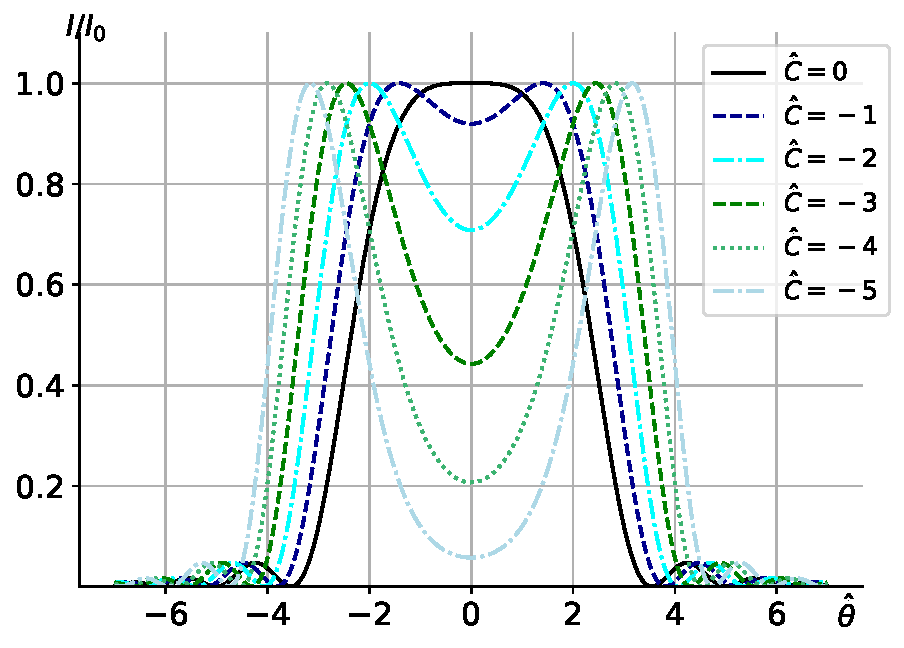
\includegraphics[width=\textwidth]{pic/angleC_neg.pdf}
		\caption{Угловое распределение поля при отрицательной сдвижке частоты}
		\label{fig:angle_dist_C_neg}
	\end{minipage}\hfill
	\begin{minipage}{0.49\textwidth}
		\centering
		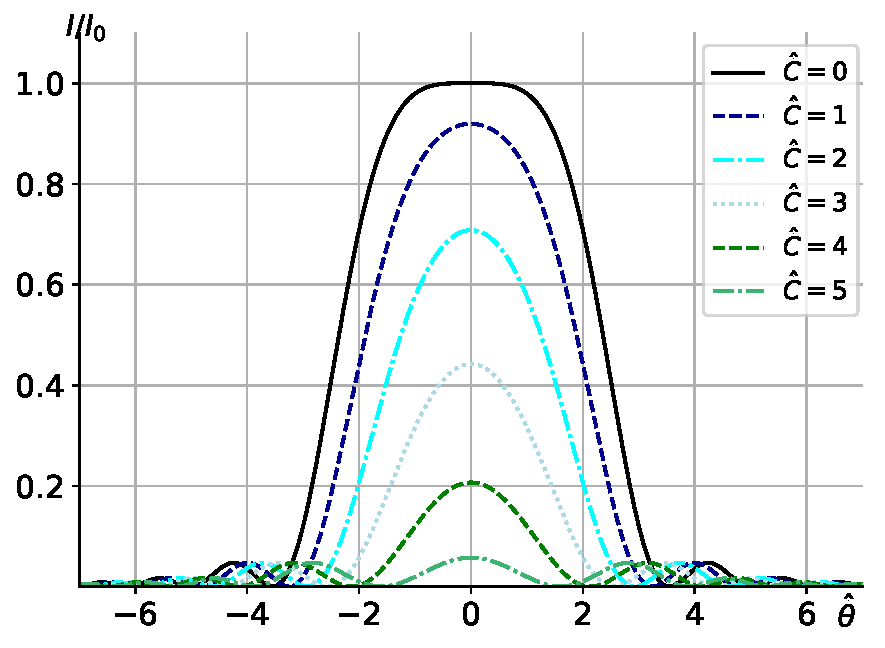
\includegraphics[width=\textwidth]{pic/angleC_pos.pdf}
		\caption{Угловое распределение поля при положительной сдвижке частоты}
		\label{fig:angle_dist_C_pos}
	\end{minipage}    
\end{figure}
\begin{figure}[h!]
	\centering
	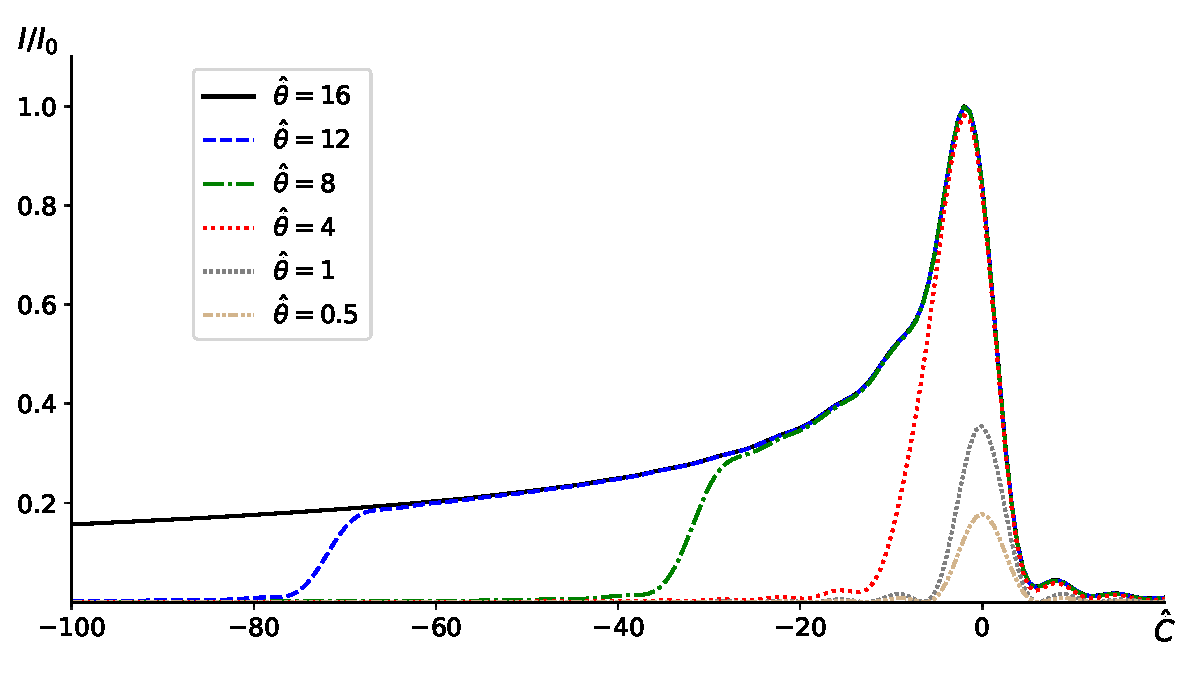
\includegraphics[width=.99\textwidth]{{pic/spec_integ_ang}.pdf}
	\caption{Проинтегрированная по углам интенсивность излучения. За $\hat{\theta}$ в легенде обозначены пределы интегрирования по углам} 
	\label{fig:spec_integrate_angle}
\end{figure}
На рис.~\ref{fig:angle_dist_C_neg} и рис.~\ref{fig:angle_dist_C_pos} изображены угловые распределения излучения. Их структуру можно понять из рисунка~\ref{fig:traj}. Конструктивная интерференция наблюдается на оси, где есть максимум интерференционной картины на резонансной частоте. Если произвести отрицательную сдвижку по частоте, то выполняется условие конструктивной интерференции: $n \lambda_{ph} = s_{ph} - \lambda_u \cos\theta$ и резонанс будет наблюдаться при ненулевых углах наблюдения. Обратно, при положительной сдвижке частоты, интенсивность быстро падает, условие резонанса не может выполниться при меньших длинах волн на ненулевых углах, потому что в набег фазы на каждом периоде ондулятора не укладывается целое число длин волн соответствующей гармоники излучения. Говорят, что электрон на каждом периоде ондулятора интерферирует сам с собой. Естественно, говорят о интерференции излучения, которое на оси обгоняет электрон на одну длину волны (или большее число волн, т.е. 1, 2, 3 и т.д. для соответствующих гармоник). На следующем периоде ондулятора электрон снова излучает в фазе с излучённой на прошлом периоде волной. Важной характеристикой в приложениях является проинтегрированный по углам $\hat{\theta}$ спектр излучения, см. рис.~\ref{fig:spec_integrate_angle}. У спектра появляется широкий "хвост". Диапазон углов по которым ведётся интегрирования и единицы измерения мощности или потока фотонов для конкретной задачи должны обсуждаться отдельно, см. Приложение~\ref{attachment:flux units}.  
\begin{figure}[htbp]
	\centering
	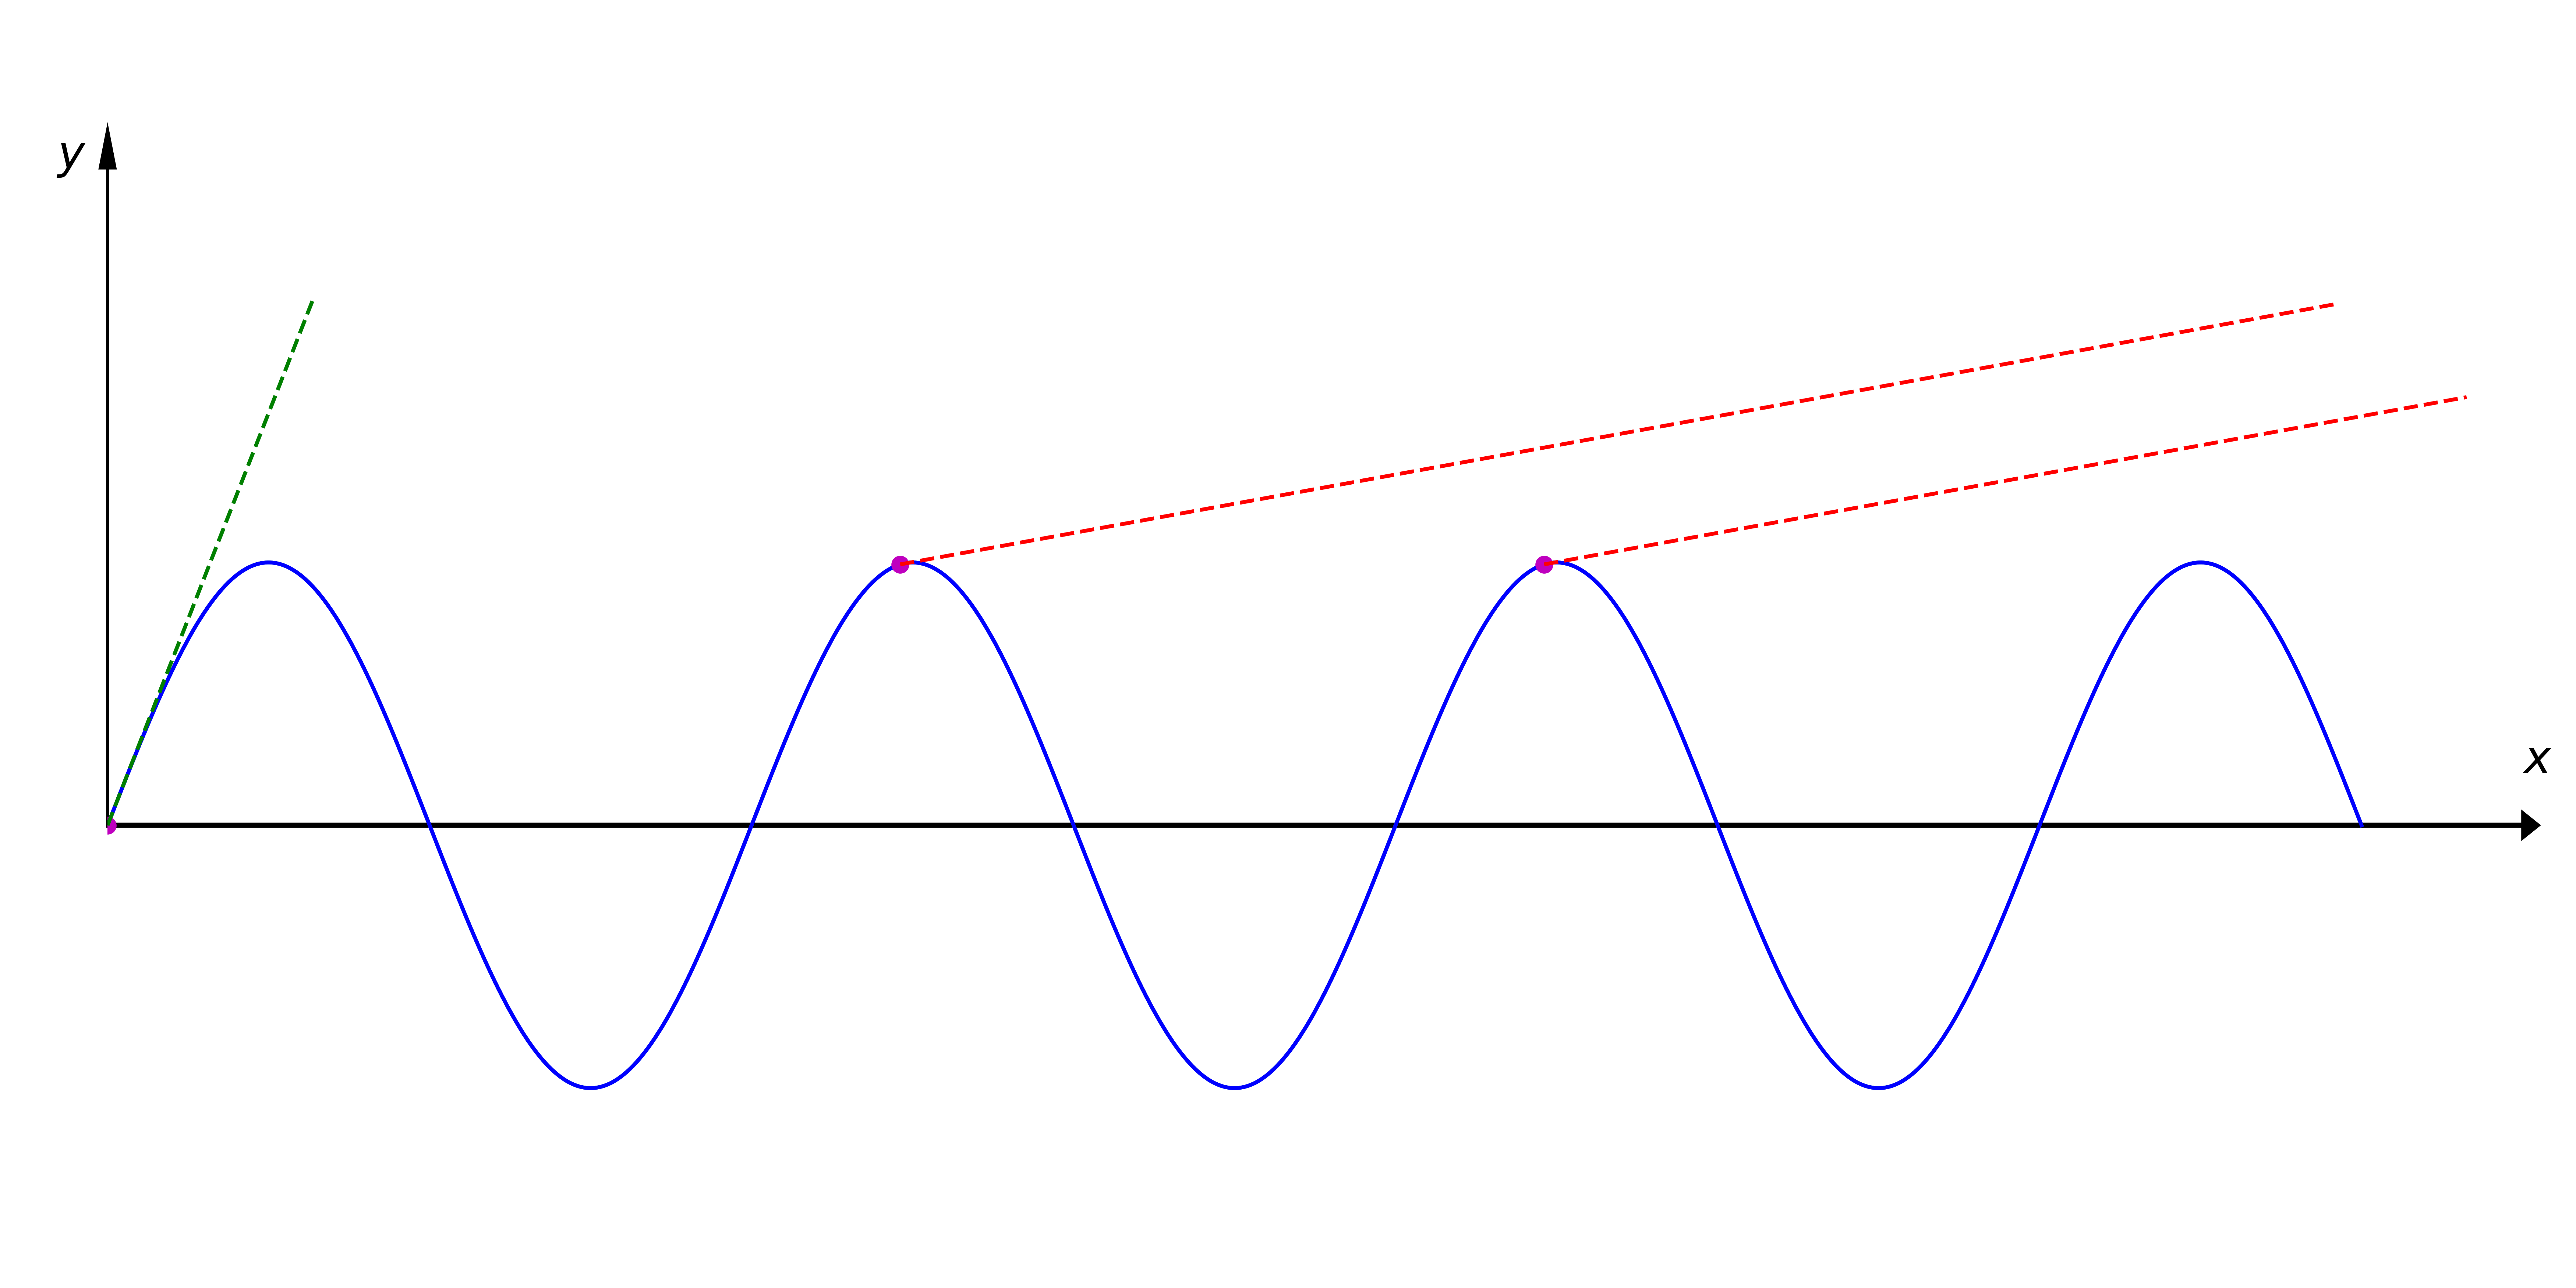
\includegraphics[width=.8\textwidth]{{pic/traj}.pdf}
	\caption{Ондулятор как интерференционное устройство} 
	\label{fig:traj}
\end{figure}

\section{Излучение высших гармоник}\label{section:HGR}
В этом разделе будет дано описание свойств излучения высших гармоник. Понимание данного вопроса необходимо в виду того, что спектральный вид излучения ондулятора сильно зависит от параметра ондуляторности $K$. Выбор этого параметра напрямую влияет на состав спектра излучения и его амплитудное распределение. Следуя выкладками~\ref{eq:field_dist_nonNorm}, где было введено обозначение $A_{JJ}$, и общей формуле для произвольной гармоники из \cite{wiedemann2015particle} можно написать:
\begin{equation}
	\label{eq:A_JJ}
	A_{JJ}(K) = \cfrac{n^2 K^2}{(1 + K^2/2)^2} \bigg[ J_{\frac{1}{2}(k-1)}\bigg(\cfrac{nK^2}{4 + 2K^2}\bigg) - J_{\frac{1}{2}(k+1)}\bigg(\cfrac{nK^2}{4 + 2K^2}\bigg)\bigg]^2,
\end{equation}
\begin{figure}[h]
	\centering 
	\begin{minipage}{0.99\textwidth}
		\centering
		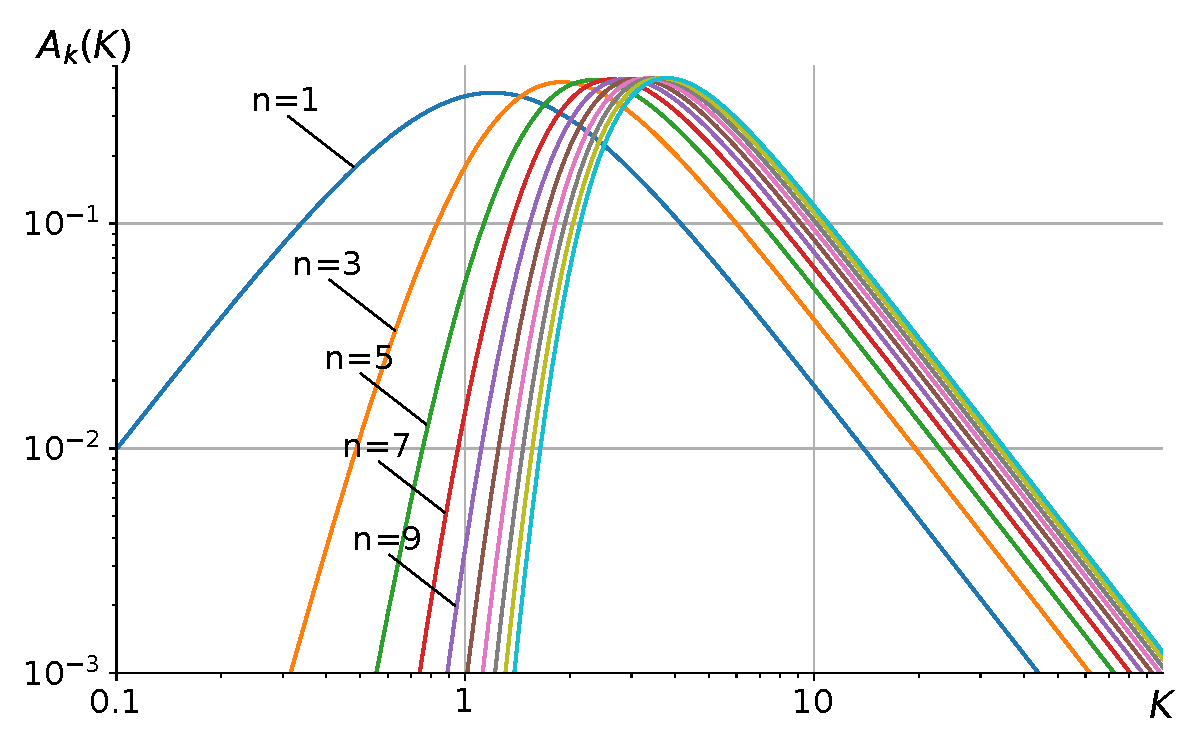
\includegraphics[width=.79\textwidth]{{pic/A_K}.pdf}
		\caption{Амплитудный спектр гармоник в зависимости от параметра ондуляторности $K$} 
		\label{fig:A_K}
	\end{minipage}
\end{figure}

Графическое представление этой формулы в зависимости от параметра $K$ показано на рис.~\ref{fig:A_K}. Спектр наглядно показывает зависимость амплитуд гармоник от параметра ондуляторности. На ондуляторах, где планируется работать на низких гармониках (1 - 7), преимущественно выбираются малые $K < 2$, если же стоят задачи использовать более высокие гармоники, то параметр $K$ выбирают в районе $2 - 2,5$.
\begin{figure}[h!]
	\begin{minipage}{0.49\textwidth}
		\centering
		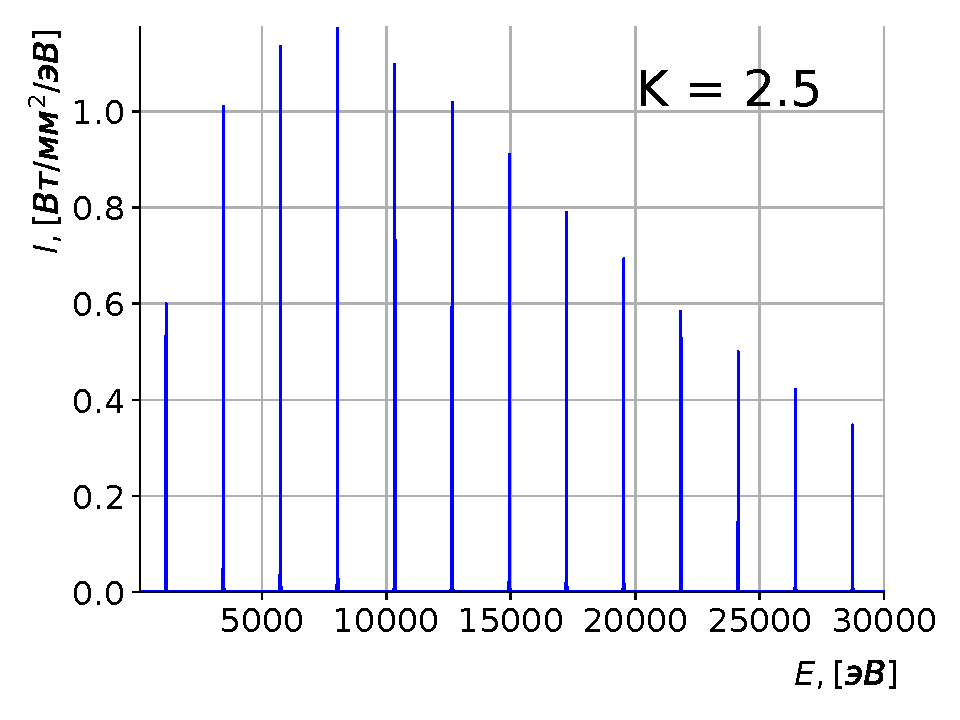
\includegraphics[width=\textwidth]{pic/spec_und_1-1.pdf}
		\caption{Спектр ондулятора с $K = 2,5$}
		\label{fig:spec_und_1-1}
	\end{minipage}
	\begin{minipage}{0.49\textwidth}
		\centering
		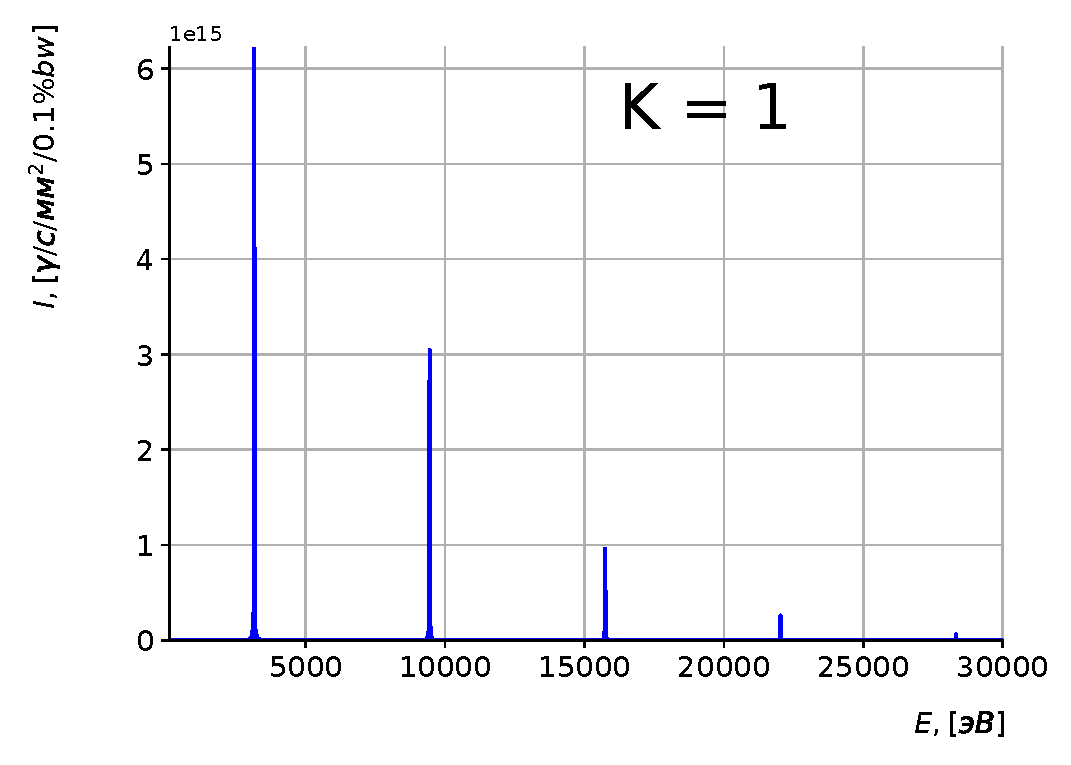
\includegraphics[width=\textwidth]{pic/spec_und_1-2.pdf}
		\caption{Спектр ондулятора с $K = 1$}
		\label{fig:spec_und_1-2}
	\end{minipage}    
\end{figure}

На рис.~\ref{fig:spec_und_1-1} и рис.~\ref{fig:spec_und_1-2} представлены примеры спектров ондуляторного излучения электронного пучка с бесконечно малым эмиттансом. Рисунки наглядно поясняют соображения изложенные выше по амплитудному составу ондуляторного спектра. Уже при при $K = 2,5$ максимум амплитуды приходиться на $7$-ую гармонику и высшие гармоники подавлены значительно слабее, по сравнению с излучением ондулятора с $K = 1$.

\section{Заключение к главе}
В главе был дан последовательный вывод свойств излучения планарного ондулятора, что даёт начальное представление необходимое для проектирования эксперементальных станции источника синхротронного излучения. Второй подход, который обычно используется в расчёте излучения релятивистского электрона основывается на использовании известных выражений для потенциалов Лиенара — Вихерта в $rt$-пространстве:
\begin{equation}
	\label{eq:Lienard_Wiechert}
	\vec{{E}}_{\bot}(\vec{r}{_0}, t) = -e \cfrac{\vec{n} - \vec{\beta}}{\gamma^2 (1 - \vec{n}\cdot\vec{\beta})^3 |\vec{r}_{ 0} - \vec{r'}|^2} - \cfrac{e}{c}\cfrac{\vec{n}\times[(\vec{n} - \vec{\beta})\times\dot{\vec{\beta}})]}{(1 - \vec{n}\cdot\vec{\beta})^3 |\vec{r}_{ 0} - \vec{r'}|}
\end{equation}
Взяв Фурье-преобразование от этого выражения по времени и совершив преобразования, описанные в \cite{geloni2006fourier}, несложно получается следующее выражение, которое является отправной точкой численных расчётов многих современных симуляционных кодов:
\begin{equation}
	\label{eq:field_dist_in_integral}
	\begin{array}{lcl}
	\vec{\widetilde{E}}_{\bot}(\vec{r}_0, \omega) = 
	-\cfrac{i\omega e}{c}\displaystyle\int\limits_{-\infty}^{\infty} dt'\bigg[\cfrac{\vec{\beta} - \vec{n}}{|\vec{r}_0 - \vec{r'}_0(t')|} - \cfrac{ic}{\omega}\cfrac{\vec{n}}{|\vec{r}_0 - \vec{r'}_0(t')|^2}\bigg]\times\\
	\\
	\exp\bigg[i\omega\bigg(t' + \cfrac{|\vec{r}_0 - \vec{r'}_0(t')|}{c}\bigg)\bigg].
	\end{array}
\end{equation}

Наиболее известный из них --- это SRW, разработанный Олегом Чубарём, \cite{chubar1998proceedings} - \cite{chubar1998accurate}. Код написан на языке $\texttt{C++}$ и является открытым кодом, что добавляет широкие возможность адаптации кода к пользовательским задачам. Методы кода позволяют рассчитывать излучение релятивистского электрона, с учётом эмиттанса, и далее пропускать получившиеся излучение через оптическую систему с применением подходов Фурье-оптики.

Другие коды и программы, которые нашли широкое применение расчёта синхротронного излучения --- это  SPECTRA \cite{SPECTRA}, XRT (XRayTracer) \cite{XRayTracer}. SPECTRA позволяет рассчитывать спектры излучения вставных устройств с широкими возможностями в выборе параметров, программа имеет доступный GUI интерфейс, и поэтому легка в использовании. XRT также имеет широкие возможности по моделированию источников синхротронного излучения, рентгенооптических трактов и оптических элементов пользовательских станций.

В работе, в основном, использовались два кода, --- SRW и SPECTRA, код XRT оставлен в стороне, т.к. возможности кода SRW вполне покрывают все потребности в расчётах, код является надёжными и проверенным инструментом при проектировании источников синхротронного излучения. 








